%% Conference version (IEEEtran, conference mode). Targets: IEEE Globecom 2027 / WiOpt 2027.
%% The journal version is journal.tex in the same project. Figures and refs.bib are shared.
\documentclass[conference]{IEEEtran}
\IEEEoverridecommandlockouts

\usepackage{cite}
\usepackage{amsmath,amssymb,amsfonts}
\let\proof\relax
\let\endproof\relax
\usepackage{amsthm}
\usepackage{algorithm}
\usepackage{algpseudocode}
\usepackage{graphicx}
\usepackage{booktabs}
\usepackage{xcolor}
\usepackage{tikz}
\usetikzlibrary{arrows.meta,positioning}

\newtheorem{assumption}{Assumption}
\newtheorem{definition}{Definition}
\newtheorem{lemma}{Lemma}
\newtheorem{proposition}{Proposition}
\newtheorem{corollary}{Corollary}
\theoremstyle{remark}
\newtheorem{remark}{Remark}

\newcommand{\E}{\mathbb{E}}
\newcommand{\Prob}{\mathbb{P}}
\newcommand{\ind}[1]{\mathbf{1}\{#1\}}
\newcommand{\A}{\mathcal{A}}
\newcommand{\G}{\mathcal{G}}
\newcommand{\I}{\mathcal{I}}
\newcommand{\lab}{\ell}
\newcommand{\Dbar}{\bar{\Delta}}
\newcommand{\ee}{\varepsilon}
\newcommand{\xh}{\hat{x}}

\begin{document}

\title{Speak When Sure, Ask When Unsure: Confidence-Aware Status Updates from On-Board UAV Classifiers}

\author{\IEEEauthorblockN{Sameh Hosny}
\IEEEauthorblockA{Akian College of Science and Engineering\\
American University of Armenia, Yerevan, Armenia\\
\{email\}}
\and
\IEEEauthorblockN{John Tadrous}
\IEEEauthorblockA{Dept.\ of Electrical and Computer Engineering\\
Gonzaga University, Spokane, WA, USA\\
tadrous@gonzaga.edu}}

\maketitle

\begin{abstract}
A UAV that classifies its imagery on board can transmit a label of a few bytes instead of a raw frame, but a small classifier errs, and a wrong label misleads the ground station. In every slot our UAV stays silent, sends its label, or uploads the raw frame to a more accurate ground classifier, with the aim of minimizing the long-run average age of incorrect information (AoII) of the ground station's status under an average energy budget and an intermittent link. Since the UAV never observes the true state, we formulate a constrained POMDP and show that a belief over the current AoII, updated with calibrated classifier confidences, is a sufficient statistic. We derive the one-step expected AoII of each action in closed form, prove that a label agreeing with the ground station's status is never worth sending, and show that the drift-plus-penalty rule reduces to confidence thresholds ordered silent, raw, label. We evaluate the resulting policy, CA-DPP, on Sentinel-2 flood-mapping traces with five-fold cross-validation over image chips and paired tests over 20 held-out runs. For budgets up to 2\,mJ per slot it lowers the average AoII by 52\% to 75\% relative to pre-identification and age-threshold policies ($p<10^{-5}$). Relative to an AoII-threshold policy, it lowers the AoII by $22\%\pm12\%$ at 0.25\,mJ per slot ($p=0.002$) and, at 0.5\,mJ per slot, by 27\% and 49\% when the on-board accuracy falls to 84\% and 82\% ($p<10^{-5}$); with an accurate classifier and ample energy the two are statistically indistinguishable.
\end{abstract}

\begin{IEEEkeywords}
Age of incorrect information, on-board inference, UAV, Lyapunov optimization, POMDP.
\end{IEEEkeywords}

%% =====================================================================
\section{Introduction}
%% =====================================================================
UAVs that monitor floods, wildfires and search areas increasingly run classifiers on board, so that a label of a few bytes can replace a video stream over a weak air-to-ground link~\cite{shamsoshoara2021flame,kyrkou2020aider}. These small models err, so a delivered update can be wrong, which the age of information misses because it resets on every delivery. The age of incorrect information (AoII)~\cite{maatouk2020aoii} grows while the receiver's estimate differs from the true state, so it penalizes wrong estimates as well as stale ones. In existing AoII work, however, the transmitter observes the source through a sensor~\cite{maatouk2020aoii,zakeri2023aoiieh,ngo2025eh}. A UAV whose sensor is a classifier knows neither the true state nor whether the ground station (GS) is currently wrong. It does know how confident its classifier is about the current frame.

The value of each update thus depends on a state the UAV cannot see, on a link whose quality changes with position, and on an energy budget shared across the mission. Our contributions are as follows.
\begin{enumerate}
\item We formulate confidence-aware status updating as a constrained POMDP that couples a calibrated per-sample error model of the on-board classifier, a ground classifier, AoII on the GS status, an intermittent link and an energy budget. A belief over the current AoII is a sufficient statistic (Sections~\ref{sec:model}--\ref{sec:problem}).
\item We derive the one-step expected AoII of each action in closed form, prove that agreeing labels have no value and that the drift-plus-penalty decision has a threshold structure in the confidence, and build the online policy CA-DPP on these results (Sections~\ref{sec:structure}--\ref{sec:lyap}).
\item We evaluate CA-DPP on Sen1Floods11 inference traces~\cite{bonafilia2020sen1floods11} under chip-level cross-validation against policies adapted from~\cite{gan2025taoi,pehlivanoglu2026orbit,basnayaka2025aomi,zakeri2023aoiieh}, and identify when per-frame confidence pays off: under tight budgets and with weak on-board classifiers (Section~\ref{sec:results}).
\end{enumerate}

%% =====================================================================
\section{Related Work}\label{sec:related}
%% =====================================================================
AoII-based updating with energy harvesting is studied in~\cite{zakeri2023aoiieh} with a POMDP and in~\cite{ngo2025eh} for random access; in both, a sensor observes the source directly. Buratto et al.~\cite{buratto2023misclass} add a misclassification penalty with a fixed error rate to offline AoI scheduling. Gan et al.~\cite{gan2025taoi} define a task-oriented AoI for cameras that pre-identify each frame and send frames containing the target to a server for re-identification; error rates are fixed. Pehlivano\u{g}lu, Li and Uysal~\cite{pehlivanoglu2026orbit} let a satellite choose among idling, on-board inference, sending a cached result and offloading raw data, and prove a threshold policy for the age of inference. Their action set is the closest to ours, but success probabilities and errors are fixed and energy is not constrained. Basnayaka et al.~\cite{basnayaka2025aomi} define the age of misclassified information for LEO event detection with a constant classification accuracy. UAV offloading~\cite{yang2020uav} and our Tiny-SEM framework~\cite{hosny2026tinysem} model classifier noise and energy queues, but not the freshness of the receiver's knowledge. Table~\ref{tab:positioning} compares these works on (E1) a per-sample, confidence-driven error model, (E2) AoII on the inferred label, (E3) an energy queue handled online, and (E4) a choice among silence, a label and raw data. No prior work combines all four.

\begin{table}[t]
\caption{Positioning. \checkmark: covered; $\circ$: partly; --: not covered.}
\label{tab:positioning}
\centering\footnotesize
\setlength{\tabcolsep}{4pt}
\begin{tabular}{@{}lcccc|lcccc@{}}
\toprule
Work & E1 & E2 & E3 & E4 & Work & E1 & E2 & E3 & E4\\
\midrule
\cite{gan2025taoi} & $\circ$ & $\circ$ & -- & $\circ$ & \cite{zakeri2023aoiieh} & -- & \checkmark & $\circ$ & $\circ$\\
\cite{pehlivanoglu2026orbit} & -- & $\circ$ & -- & \checkmark & \cite{buratto2023misclass} & $\circ$ & \checkmark & -- & --\\
\cite{basnayaka2025aomi} & $\circ$ & $\circ$ & -- & -- & \cite{yang2020uav} & $\circ$ & -- & $\circ$ & $\circ$\\
\midrule
This work & \checkmark & \checkmark & \checkmark & \checkmark & & & & & \\
\bottomrule
\end{tabular}
\end{table}

%% =====================================================================
\section{System Model}\label{sec:model}
%% =====================================================================
\begin{figure}[t]
\centering
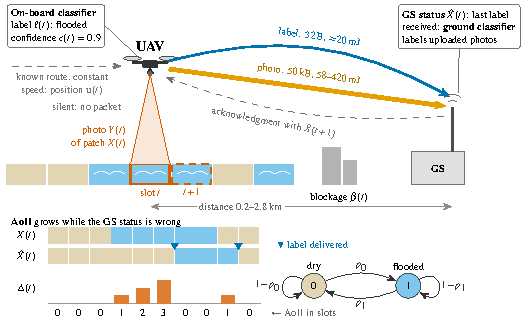
\includegraphics[width=\columnwidth]{figures/fig_scenario_conf.pdf}
\caption{The UAV labels each photo on board, then stays silent, sends its label (blue), or sends the photo to the ground classifier (orange). The GS status is the last label received. Bottom: the AoII grows while the GS status is wrong; right: the Markov chain of $X(t)$.}
\label{fig:system}
\end{figure}

We consider a UAV that surveys a disaster area, such as a flood, for a ground station (GS) that guides rescue teams (Fig.~\ref{fig:system}). The GS has no sensor of its own: its status for the patch below the UAV is the last label it received, sent by the UAV or produced by the GS classifier from a photo the UAV sent, and it holds this status until the next update. The UAV flies a known route at constant speed, so its position $\mathbf{u}(t)$ is known in advance. In each slot $t\in\{0,1,\dots\}$ of length $\tau$ it photographs the patch below it and labels it on board. It then stays silent, sends its label, which is cheap but makes a correct GS status wrong if the label is wrong, or sends the photo, which is reliable but costly. It never sees whether the GS status is wrong. Table~\ref{tab:notation} lists the notation.

\subsection{Source and Inference}
The scene state is $X(t)=1$ if the event is present (here, flooded) and $X(t)=0$ otherwise (dry); labels and the GS status use the same convention. It refers to the patch below the UAV in slot $t$, not to a fixed patch, and evolves along the route as a Markov chain (Fig.~\ref{fig:system}) with
\begin{equation}\label{eq:source}
\Prob\big\{X(t+1)\neq x\mid X(t)=x\big\}=p_x,\qquad 0<p_0,p_1<\tfrac12 .
\end{equation}
Thus $p_x$ describes changes between consecutive footprints and depends on the speed and the footprint overlap. Let $\varpi_x$ be the stationary law of this chain. The chain may be asymmetric; in our data flooded footprints turn dry more often than dry ones flood ($p_1>p_0$). We use the symmetric case $p_0=p_1$ only to state closed forms. In slot $t$ the UAV captures a frame $Y(t)$, and its classifier outputs a label $\lab(t)$ and a confidence $c(t)\in[\tfrac12,1]$, the probability it gives that label. After a raw upload, the GS classifier returns a label $\lab^{\rm g}(t)$.

\begin{assumption}[Inference model]\label{as:inf}
(i) The on-board classifier is calibrated with respect to the prior $\varpi$: $\Prob\{X(t)=\lab(t)\mid\lab(t),c(t)\}=c(t)$, so $\Prob\{\lab(t)\neq X(t)\mid c(t)=c\}=1-c$. (ii) Given the source path, the outputs $(\lab(t),c(t))$ are independent across slots. (iii) Given $X(t)$ and $c(t)=c$, the ground label is wrong with probability $\ee_{\rm g}(c)<\tfrac12$, independently of $\lab(t)$.
\end{assumption}

Post-hoc calibration~\cite{guo2017calibration} makes (i) hold approximately; our on-board model has an expected calibration error of $1.2\%$. By (i), which must hold for each label value and not only on average, Bayes' rule makes the likelihood of the frame under $X(t)=x$ proportional to $\Prob\{X(t)=x\mid\lab(t),c(t)\}/\varpi_x$. Dividing by $\varpi_x$ avoids counting the class prior twice, once inside the classifier and once in the source dynamics, and it lets the belief account for errors that are more frequent in one class than in the other. Part (ii) is optimistic for imagery because consecutive footprints overlap; we correct for this below. Part (iii) lets the ground error depend on $c$, since frames that are hard on board are often hard on the ground: in our data the ground model errs on $20\%$ of the frames the on-board model gets wrong and on $0.8\%$ of the others. Assumption~\ref{as:inf} is used only by the controller; the simulations replay real, correlated labels. It generalizes the semantic-noise model of Tiny-SEM~\cite{hosny2026tinysem} by letting the noise level vary per sample.

\subsection{Actions, Link and Energy}
At the start of slot $t$ the UAV chooses $a(t)\in\A=\{0,1,2\}$: silence, the label in $L_1$ bits, or the frame in $L_2\gg L_1$ bits. The channel state $g(t)=(\mathbf{u}(t),\beta(t))$ holds the UAV position, which affects only the link, and a blockage indicator $\beta(t)$, which follows a two-state Markov chain with $\Prob\{\beta(t+1)=1\mid\beta(t)=0\}=\rho_{\rm b}$ and $\Prob\{\beta(t+1)=0\mid\beta(t)=1\}=\rho_{\rm u}$. Following~\cite{alhourani2014lap}, the mean path loss at elevation angle $\phi$ and distance $r$ is
\begin{equation}\label{eq:pl}
\overline{\rm PL}(r,\phi)={\rm FSPL}(r)+P_{\rm LoS}(\phi)\,\eta_{\rm LoS}+\big(1-P_{\rm LoS}(\phi)\big)\eta_{\rm NLoS},
\end{equation}
with $P_{\rm LoS}(\phi)=[1+\alpha e^{-b(\phi-\alpha)}]^{-1}$, which gives the mean SNR $\bar\gamma(g)$. With Rayleigh block fading, bandwidth $W$ and a rateless code sent until acknowledged or for at most $\tau_{\max}\le\tau$, a packet of $L_a$ bits is decoded with probability
\begin{equation}\label{eq:succ}
q_a(g)=(1-\beta)\exp\big(-(2^{L_a/(W\tau_{\max})}-1)/\bar\gamma(g)\big),
\end{equation}
so $q_2(g)\le q_1(g)$, and $q_0\equiv0$. The link is an erasure channel: a packet with a failed CRC is discarded and leaves the GS status unchanged. A transmission costs $E_a(g)=P_{\rm r}\min\{L_a/\bar R(g),\tau_{\max}\}+E_{\rm o}$ for $a\in\{1,2\}$, with mean rate $\bar R(g)=W\log_2(1+\bar\gamma(g))$ (fading changes the raw cost by $-10\%$ to $+42\%$), radio power $P_{\rm r}$ and per-packet overhead $E_{\rm o}$ (wake-up, access and acknowledgment), and $E_0=0$. Capture and inference cost the same in every slot and do not affect the decision. Propulsion energy depends on the trajectory~\cite{zeng2019rotary}, not on our decisions, so we constrain only the communication energy:
\begin{equation}\label{eq:budget}
\limsup_{T\to\infty}\tfrac1T\textstyle\sum_{t<T}\E\Big[E_{a(t)}\big(g(t)\big)\Big]\le\bar E.
\end{equation}

\subsection{GS Status and AoII}
Let $o(t)\in\{0,1\}$ indicate that the packet of slot $t$ is decoded, so $\Prob\{o(t)=1\mid a(t)=a,g(t)=g\}=q_a(g)$. The GS status evolves as
\begin{equation}\label{eq:est}
\hat X(t+1)=\begin{cases}\lab(t), & a(t)=1,\ o(t)=1,\\ \lab^{\rm g}(t), & a(t)=2,\ o(t)=1,\\ \hat X(t), & \text{otherwise.}\end{cases}
\end{equation}
Every decoded packet is acknowledged with $\hat X(t+1)$ (one byte), so the UAV knows $\hat X(t)$ but never $X(t)$. After the scene moves to $X(t+1)$, the AoII is
\begin{equation}\label{eq:aoii}
\Delta(t+1)=\big(\Delta(t)+1\big)\,\ind{X(t+1)\neq\hat X(t+1)},\quad \Delta(0)=0.
\end{equation}
In slot $t$ the events occur in this order: the UAV observes $g(t)$, captures $Y(t)$ and computes $(\lab(t),c(t))$; it chooses $a(t)$; the packet is decoded with probability $q_{a(t)}(g(t))$ and the GS updates its status by~\eqref{eq:est} and acknowledges; finally the scene moves to $X(t+1)$ and $\Delta(t+1)$ follows~\eqref{eq:aoii}.

%% =====================================================================
\section{Problem Formulation}\label{sec:problem}
%% =====================================================================
\subsection{Information and Objective}
When the UAV chooses $a(t)$, it knows
\begin{equation}\label{eq:info}
\I(t)=\big\{\lab(s),c(s),g(s)\big\}_{s\le t}\cup\big\{a(s),\hat X(s+1)\big\}_{s<t}
\end{equation}
and the ground label of each decoded upload, but not $X(t)$ or $\Delta(t)$. A policy $\psi$ maps $\I(t)$ to a distribution on $\A$, with $a(t)=0$ whenever $q_1(g(t))=0$. The GS status should be wrong as rarely and as briefly as possible, which the average AoII measures, within the budget:
\begin{equation}\label{eq:P}
\textbf{(P)}\quad \min_{\psi}\ \limsup_{T\to\infty}\tfrac1T\textstyle\sum_{t<T}\E^{\psi}\big[\Delta(t)\big]\quad\text{s.t. \eqref{eq:budget}}.
\end{equation}
(P) is hard: its cost depends on the unobserved $X(t)$, the AoII has memory, and the budget couples all slots. A belief on the AoII removes the first difficulty.

\subsection{Belief on the AoII}\label{sec:belief}
\begin{lemma}[Sufficient statistic]\label{lem:suff}
Given $\hat X(t)$, $X(t)=\hat X(t)$ if $\Delta(t)=0$ and $X(t)=1-\hat X(t)$ otherwise. Hence $\hat X(t)$ and the belief $\pi_t(\delta)=\Prob\{\Delta(t)=\delta\mid\I(t)\}$ summarize $\I(t)$ for predicting future AoII.
\end{lemma}
\begin{proof}
By~\eqref{eq:aoii}, $\Delta(t)>0$ iff $X(t)\neq\hat X(t)$, and $X(t)$ is binary.
\end{proof}

We truncate the support at $\Delta_{\max}$ and keep the mass that would exceed $\Delta_{\max}$ at $\Delta_{\max}$. Let $\pi^-_t$ be the belief before the new label is seen, $d(t)=\ind{\lab(t)\neq\hat X(t)}$, and $x_\delta$ the scene state implied by $\delta$ (Lemma~\ref{lem:suff}). The recursion has three steps.

\emph{Correction with the on-board label.} All $\delta>0$ imply the same state, so only the likelihood ratio $\Lambda_t$ of ``GS wrong'' to ``GS right'' matters. By (i), with $\xh=\hat X(t)$,
\begin{equation}\label{eq:Lambda}
\Lambda_t=\frac{\varpi_{\xh}}{\varpi_{1-\xh}}\times\begin{cases}c(t)/\big(1-c(t)\big), & d(t)=1,\\ \big(1-c(t)\big)/c(t), & d(t)=0.\end{cases}
\end{equation} The controller updates
\begin{equation}\label{eq:post}
\pi_t(\delta)\propto\pi^-_t(\delta)\,\Lambda_t^{\nu\ind{\delta>0}},
\end{equation}
which multiplies the odds that the GS is wrong by $\Lambda_t^{\nu}$. Overlapping footprints violate part (ii), so instead of Bayes' rule ($\nu=1$) we temper the evidence with $\nu\in(0,1]$, which counts each frame as a fraction $\nu$ of an independent observation. With $\varpi_0=\varpi_1$ and $\nu=1$, \eqref{eq:post} is the symmetric update in which $c(t)$ itself is the likelihood. We select $\nu$ on tuning data together with the other controller parameters.

\emph{Correction with the ground label.} After a decoded raw upload, \eqref{eq:post} applies with $\nu=1$ and $\Lambda_t=(1-\ee_{\rm g})/\ee_{\rm g}$ if $\lab^{\rm g}(t)\neq\hat X(t)$, or its inverse otherwise, with $\ee_{\rm g}=\ee_{\rm g}(c(t))$.

\emph{Prediction.} Let $\xh'=\hat X(t+1)$. Since $x_\delta$ is known for each $\delta$, so is whether $X(t)=\xh'$, and
\begin{equation}\label{eq:pred}
\Prob\big\{\Delta(t+1)=\delta+1\mid\Delta(t)=\delta\big\}=\begin{cases}p_{x_\delta}, & x_\delta=\xh',\\ 1-p_{x_\delta}, & x_\delta\neq\xh',\end{cases}
\end{equation}
with $\Delta(t+1)=0$ otherwise. This gives $\pi^-_{t+1}$.

We use $\mu_t=\pi_t(\Delta>0)$, the probability that the GS is wrong, and $S_t=\E_{\pi_t}[(\Delta+1)\ind{\Delta>0}]$, and write $\mu^-_t$, $S^-_t$ for the same quantities under $\pi^-_t$.

\begin{table}[t]
\caption{Main notation}\label{tab:notation}
\centering\footnotesize
\begin{tabular}{@{}ll@{}}
\toprule
$X(t)$, $\hat X(t)$ & true state; GS status \\
$p_0,p_1$; $\varpi_x$ & source transition probabilities; stationary law \\
$\lab(t)$, $c(t)$; $d(t)$ & on-board label, confidence; disagreement with GS \\
$\Lambda_t$; $\nu$ & evidence that GS is wrong; its discount \\
$\ee_{\rm g}(c)$ & ground error probability \\
$a(t)$ & action: 0 silent, 1 label, 2 raw \\
$g(t)$, $q_a(g)$, $E_a(g)$ & link state; delivery probability; energy \\
$\Delta(t)$; $\pi_t$ & AoII of the GS status; belief on $\Delta(t)$ \\
$\mu_t$, $S_t$ & $\Prob$(GS wrong); $\E[(\Delta{+}1)\ind{\Delta>0}]$ \\
$\bar E$, $Z(t)$, $V$ & energy budget; virtual queue; DPP weight \\
\bottomrule
\end{tabular}
\end{table}

By Lemma~\ref{lem:suff}, (P) is a constrained MDP on the state $(\pi^-_t,\hat X(t),\lab(t),c(t),g(t))$ with per-slot cost $\E[\Delta(t+1)\mid\I(t),a(t)]$ and energy $E_{a(t)}(g(t))$. Its kernel follows from the model and the recursion above. A multiplier $\lambda\ge0$ on the energy constraint turns (P) into an unconstrained average-cost problem with cost $\E[\Delta(t+1)]+\lambda E_{a(t)}$. Solving it requires value iteration over a continuous belief simplex and knowledge of the confidence distribution, the blockage statistics and the trajectory. These are hard to obtain before a mission, and the computation does not fit on board. We therefore characterize the per-slot decision in closed form and build an online policy on it.

%% =====================================================================
\section{Structure of the Per-Slot Decision}\label{sec:structure}
%% =====================================================================
Fix slot $t$, let $\xh=\hat X(t)$, and let $r=p_{\xh}$ and $w=p_{1-\xh}$.

\begin{lemma}[One-step expected AoII]\label{lem:onestep}
Under Assumption~\ref{as:inf}, given $\I(t)$ and delivery, the expected AoII in slot $t+1$ is $J_0$ under silence, $J_1$ after a label and $J_2$ after a raw upload:
\begin{align*}
J_0&=(1-\mu_t)\,r+S_t\,(1-w),\\
J_1&=(1-\mu_t)(1-r)+S_t\,w\quad\text{if } d(t)=1,\\
J_2&=(1-\mu_t)\big[r+\ee_{\rm g}(1-2r)\big]+S_t\big[w+\ee_{\rm g}(1-2w)\big],
\end{align*}
and $J_1=J_0$ if $d(t)=0$. Hence $\E[\Delta(t+1)\mid\I(t),a]=J_0-q_a(g)\,G_a$, with $G_0=0$ and
\begin{align}
G_1&=\big[S_t(1-2w)-(1-\mu_t)(1-2r)\big]\,d(t), \label{eq:G1}\\
G_2&=(1-\ee_{\rm g})\,S_t(1-2w)-\ee_{\rm g}\,(1-\mu_t)(1-2r). \label{eq:G2}
\end{align}
\end{lemma}
\begin{proof}
Given $\Delta(t)=\delta$ and $\hat X(t+1)$, $\E[\Delta(t+1)]$ is $\delta+1$ times the probability in~\eqref{eq:pred}. Under silence this probability is $r$ for $\delta=0$ and $1-w$ for $\delta>0$; averaging over $\pi_t$ gives $J_0$. A delivered disagreeing label flips the GS status, so it becomes $1-r$ and $w$. A delivered ground label equals $X(t)$ with probability $1-\ee_{\rm g}$, independently of $\Delta(t)$ given $c(t)$, which mixes the two cases. Subtracting gives~\eqref{eq:G1} and~\eqref{eq:G2}.
\end{proof}

The term $S_t(1-2w)$ is the AoII removed when the GS is wrong and the update is right, and $(1-\mu_t)(1-2r)$ is the AoII created when the GS is right and the update is wrong. A delivered label always removes the first term, since a label that disagrees with a wrong GS is correct, and always creates the second. A ground label removes the first term only with probability $1-\ee_{\rm g}$ and creates the second only with probability $\ee_{\rm g}$. A label that is probably wrong has $G_1<0$.

\begin{corollary}[Symmetric source]\label{cor:sym}
If $p_0=p_1=p$, then $G_1=(1-2p)(\Dbar_t+2\mu_t-1)\,d(t)$ and $G_2=(1-2p)\big(\mu_t+(1-\ee_{\rm g})\Dbar_t-\ee_{\rm g}\big)$, where $\Dbar_t=\E_{\pi_t}[\Delta(t)]$.
\end{corollary}

\begin{proposition}[No confirmations]\label{prop:confirm}
If $d(t)=0$, then $G_1=0$, so a policy that minimizes expected AoII plus a nonnegative energy price never sends a label that agrees with the GS.
\end{proposition}

Consider any per-slot rule with weight $V>0$ and energy price $\lambda(t)\ge0$,
\begin{equation}\label{eq:rule}
a(t)\in\arg\max_{a\in\A}\big\{V\,q_a(g)\,G_a-\lambda(t)\,E_a(g)\big\}.
\end{equation}

The confidence enters the gains only through $\Lambda_t$, which increases in $c$ if $d(t)=1$ and decreases if $d(t)=0$.

\begin{lemma}\label{lem:mono}
Fix $\pi^-_t$. For $A,B\ge0$, $AS_t-B(1-\mu_t)$ is nondecreasing in $\Lambda_t$.
\end{lemma}
\begin{proof}
Let $y=\Lambda_t^{\nu}$. By~\eqref{eq:post}, $S_t=yS^-_t/D$ and $1-\mu_t=(1-\mu^-_t)/D$ with $D=1-\mu^-_t+\mu^-_ty$. So $AS_t-B(1-\mu_t)=N/D$ with $N$, $D$ affine in $y$, and $N'D-ND'=(1-\mu^-_t)(AS^-_t+B\mu^-_t)\ge0$.
\end{proof}

\begin{proposition}[Confidence thresholds]\label{prop:threshold}
Let $\ee_{\rm g}$ be constant and fix $\pi^-_t$, $\hat X(t)$, $g$ and $\lambda(t)$. (a) If $d(t)=1$, there are $c_{\rm r}\le c_{\lab}$ such that \eqref{eq:rule} stays silent for $c<c_{\rm r}$, uploads raw data for $c_{\rm r}\le c<c_{\lab}$ and sends the label for $c\ge c_{\lab}$ (any interval may be empty). (b) If $d(t)=0$, it uploads raw data iff $c\le c^0_{\rm r}$ for some $c^0_{\rm r}$. (c) For fixed $\mu^-_t$, the silent regions shrink as $S^-_t$ grows and grow with $\lambda(t)$.
\end{proposition}
\begin{proof}
Let $f_a=Vq_aG_a-\lambda E_a$. Since $r,w<\tfrac12$, $G_1$, $G_2$ have the form $AS_t-B(1-\mu_t)$ with $A,B\ge0$. So does $q_1G_1-q_2G_2$, with $A=(1-2w)(q_1-q_2(1-\ee_{\rm g}))$ and $B=(1-2r)(q_1-q_2\ee_{\rm g})$, both nonnegative as $q_2\le q_1$. By Lemma~\ref{lem:mono}, $f_2-f_0$ and $f_1-f_2$ are nondecreasing in $\Lambda_t$. For $d=1$, $\Lambda_t$ increases in $c$, so $f_a$ has increasing differences in $(a,c)$ for the order $0\prec2\prec1$, and Topkis' theorem gives (a). For $d=0$, Proposition~\ref{prop:confirm} excludes the label and $f_2-f_0$ is nonincreasing in $c$, giving (b). For (c), $S^-_t$ enters $N$ with coefficient $Ay\ge0$, and each $f_a-f_0$ ($a\neq0$) decreases in $\lambda$.
\end{proof}

\begin{figure}[t]
\centering
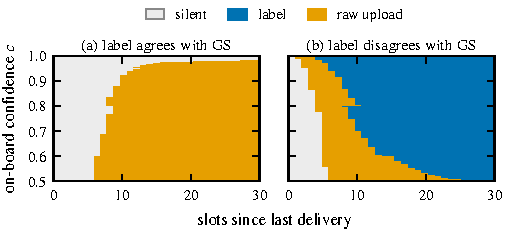
\includegraphics[width=\columnwidth]{figures/regions.pdf}
\caption{Decisions of~\eqref{eq:rule} versus the slots since the last delivery and the confidence, with parameters estimated on Sen1Floods11: GS reports ``not flooded'' with $5\%$ initial doubt, UAV $1.2$\,km from the GS ($q_1\approx1$, $q_2=0.78$, $E_1=20$\,mJ, $E_2=190$\,mJ), $\lambda/V=2$\,J$^{-1}$, $\nu=0.25$.}
\label{fig:regions}
\end{figure}

Fig.~\ref{fig:regions} evaluates~\eqref{eq:rule} with the confidence-dependent $\ee_{\rm g}(c)$ estimated from our data, which Proposition~\ref{prop:threshold} does not cover; the order silent, raw, label still holds. When the label disagrees with the GS, the confidence needed to send it falls as the GS status ages. When the label agrees but is uncertain, the UAV uploads the frame once the status is old enough, which amounts to asking the GS to verify.

\begin{table*}[t]
\caption{Trace-driven results at two energy budgets (mean $\pm$ 95\% confidence half-width over 20 held-out runs: 5-fold cross-validation over chips, 4 runs per fold). $\Delta$: change in average AoII obtained by CA-DPP relative to the policy in that row (negative means CA-DPP is lower), with paired 95\% confidence interval, paired $t$-test $p$-value, and the number of folds (out of 5) in which CA-DPP has the lower mean.}
\label{tab:results}
\centering\footnotesize\setlength{\tabcolsep}{3.2pt}
\begin{tabular}{@{}lcccccccc@{}}
\toprule
 & \multicolumn{4}{c}{$\bar E=0.25$\,mJ/slot} & \multicolumn{4}{c}{$\bar E=2$\,mJ/slot}\\
\cmidrule(lr){2-5}\cmidrule(l){6-9}
Policy & AoII & $\Delta$ (\%) & $p$ & folds & AoII & $\Delta$ (\%) & $p$ & folds\\
\midrule
CA-DPP (proposed) & $0.645\pm0.165$ & -- & -- & -- & $0.390\pm0.085$ & -- & -- & -- \\
AoII threshold~\cite{zakeri2023aoiieh} & $0.925\pm0.258$ & $-22.3\pm11.6$ & $0.002$ & 4/5 & $0.352\pm0.060$ & $+9.5\pm13.2$ & $0.171$ & 3/5 \\
Pre-identification~\cite{gan2025taoi} & $2.556\pm0.284$ & $-74.8\pm6.2$ & $<\!10^{-3}$ & 5/5 & $0.796\pm0.129$ & $-52.0\pm5.2$ & $<\!10^{-3}$ & 5/5 \\
Age threshold~\cite{pehlivanoglu2026orbit} & $2.538\pm0.381$ & $-74.8\pm4.2$ & $<\!10^{-3}$ & 5/5 & $0.784\pm0.114$ & $-51.8\pm5.1$ & $<\!10^{-3}$ & 5/5 \\
Always offload~\cite{basnayaka2025aomi} & $12.451\pm1.288$ & $-94.5\pm1.5$ & $<\!10^{-3}$ & 5/5 & $8.444\pm0.869$ & $-95.2\pm1.1$ & $<\!10^{-3}$ & 5/5 \\
\midrule
CA-DPP, confidence-blind & $0.739\pm0.165$ & $-13.3\pm5.2$ & $0.001$ & 4/5 & $0.345\pm0.056$ & $+10.3\pm9.9$ & $0.051$ & 2/5 \\
CA-DPP, label only & $0.686\pm0.204$ & $+6.7\pm13.8$ & $0.487$ & 1/5 & $0.428\pm0.101$ & $-7.1\pm3.0$ & $0.001$ & 4/5 \\
\midrule
Genie (knows $X$) & \multicolumn{8}{l}{AoII $0.171\pm0.011$, $\Prob$(GS wrong) $0.070$, energy $0.96$\,mJ/slot when unconstrained} \\
\bottomrule
\end{tabular}
\end{table*}

%% =====================================================================
\section{Online Policy: CA-DPP}\label{sec:lyap}
%% =====================================================================
We enforce~\eqref{eq:budget} with the virtual queue $Z(t+1)=\max\big\{Z(t)+E_{a(t)}(g(t))-\bar E,0\big\}$, $Z(0)=0$, whose mean-rate stability implies~\eqref{eq:budget}~\cite{neely2010book}. With $L(t)=\tfrac12Z(t)^2$,
\begin{equation}\label{eq:drift}
\begin{split}
&\E\big[L(t+1)-L(t)\,|\,\I(t)\big]\\
&\qquad\le C+Z(t)\,\E\Big[E_{a(t)}\big(g(t)\big)-\bar E\,\Big|\,\I(t)\Big],
\end{split}
\end{equation}
where $C=\tfrac12\max\{E_{\max},\bar E\}^2$ and $E_{\max}=\max_{a,g}E_a(g)$. CA-DPP minimizes the right-hand side of~\eqref{eq:drift} plus $V\,\E[\Delta(t+1)\mid\I(t),a]$, which by Lemma~\ref{lem:onestep} is rule~\eqref{eq:rule} with $\lambda(t)=Z(t)$. Algorithm~\ref{alg:dpp} lists the steps. A slot costs $O(\Delta_{\max})$ operations, less than one inference.

\begin{algorithm}[t]
\caption{CA-DPP, executed by the UAV in slot $t$}\label{alg:dpp}
\begin{algorithmic}[1]
\State Classify $Y(t)$ to get $(\lab(t),c(t))$; observe $g(t)$; set $d(t)$
\State Correct $\pi^-_t\to\pi_t$ by~\eqref{eq:post}; compute $\mu_t$, $S_t$, $G_1$, $G_2$
\State $a(t)\gets\arg\max_a\{Vq_a(g)G_a-Z(t)E_a(g)\}$ (silent if $q_1(g)=0$)
\State Transmit; read the acknowledgment ($\hat X(t+1)$, and $\lab^{\rm g}(t)$ after a raw upload)
\State If a raw upload was decoded, correct $\pi_t$ with $\lab^{\rm g}(t)$; predict $\pi^-_{t+1}$
\State $Z(t+1)\gets\max\big\{Z(t)+E_{a(t)}(g(t))-\bar E,0\big\}$
\end{algorithmic}
\end{algorithm}

\begin{remark}[Harvesting battery]
If the UAV or a ground node harvests energy into a battery with content $B(t)$, the same derivation with the battery shifted by a constant $\theta$~\cite{huang2013eh} gives~\eqref{eq:rule} with $\lambda(t)=\theta-B(t)$. Since $q_aG_a\le S_t\le\Delta_{\max}+1$, choosing $\theta\ge E_{\max}+V(\Delta_{\max}+1)/E_{\min}$, with $E_{\min}=\min_{a\neq0,g}E_a(g)$, keeps every action within the battery content.
\end{remark}

\begin{remark}[Performance]
The $O(1/V)$ optimality gap of drift-plus-penalty~\cite{neely2010book} assumes that per-slot costs do not depend on past decisions, which does not hold for AoII. A version that applies~\eqref{eq:rule} between deliveries fits the renewal framework of~\cite{neely2013renewal}; we leave its analysis to future work.
\end{remark}

%% =====================================================================
\section{Trace-Driven Evaluation}\label{sec:results}
%% =====================================================================

\begin{figure*}[t]
\centering
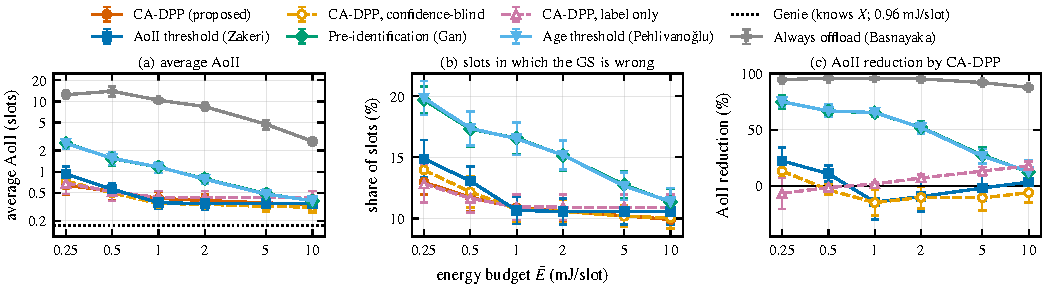
\includegraphics[width=\textwidth]{figures/fig_budget.pdf}
\caption{Energy budget sweep, $20$ held-out runs per point, with $95\%$ confidence intervals. (a) Average AoII. (b) Fraction of slots in which the GS is wrong. (c) AoII reduction by CA-DPP relative to each policy (paired intervals); negative values favor the other policy.}
\label{fig:budget}
\end{figure*}

\begin{figure*}[t]
\centering
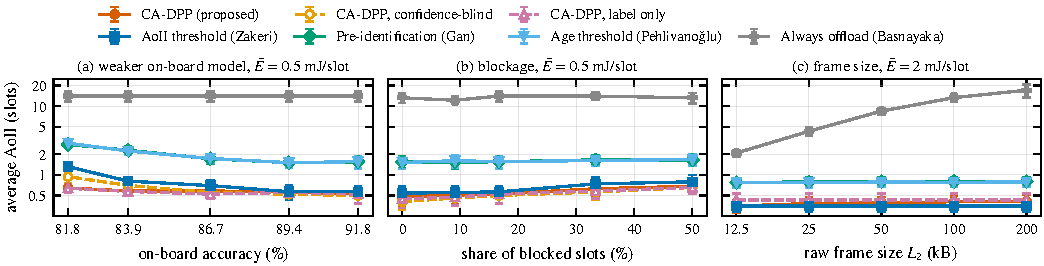
\includegraphics[width=\textwidth]{figures/fig_sensitivity.pdf}
\caption{Sensitivity ($20$ runs per point): (a) on-board accuracy and (b) share of blocked slots, $\rho_{\rm b}/(\rho_{\rm b}+\rho_{\rm u})$, at $\bar E=0.5$; (c) raw frame size at $\bar E=2$\,mJ/slot.}
\label{fig:sens}
\end{figure*}

\subsection{Data, Classifiers and Scenario}
We build traces from the hand-labeled part of Sen1Floods11~\cite{bonafilia2020sen1floods11}: 446 Sentinel-2 chips of $512\times512$ pixels at $10$\,m from eleven flood events, with official train, validation and test splits. A $64\times64$-pixel footprint scans each chip along a serpentine path with a stride of $32$ pixels, one footprint per slot, and is labeled flooded if at least $10\%$ of its labeled pixels are water. Footprints with less than $80\%$ labeled pixels are skipped, which leaves $46{,}774$, $16{,}612$ and $16{,}811$ slots in the three splits. Consecutive footprints overlap, so the state sequence is strongly correlated; on the training split $p_0=0.039$ and $p_1=0.166$. We use this Sentinel-2 imagery as a proxy for the UAV's downward view.

The on-board model is a logistic regression on the $8\times8$ average-pooled blue, green, red and near-infrared bands (257 parameters). The ground model is a gradient-boosted tree ensemble (300 trees) on 77 statistics of all 13 bands and two water indices. Both are trained on the training split and calibrated by isotonic regression on the validation split. To vary the on-board quality, we add Gaussian noise of $2$, $4$, $6$ and $8$ times the per-band standard deviation to its input and recalibrate. On the $174$ validation and test chips ($33{,}423$ slots, $20.5\%$ flooded), the five on-board variants are correct on $91.8\%$, $89.4\%$, $86.7\%$, $83.9\%$ and $81.8\%$ of the slots, and the ground model on $97.6\%$. Noise makes the on-board errors lopsided: the noisiest variant labels $7\%$ of the test slots as flooded, against $21\%$ in truth.

The UAV flies at $100$\,m on a circle of radius $1.3$\,km centered $1.5$\,km from the GS, so its distance to the GS ranges from $0.2$ to $2.8$\,km over one orbit of $400$ slots ($\tau=0.5$\,s). The link uses $2.4$\,GHz, $W=1$\,MHz, $20$\,dBm, a $7$\,dB noise figure and the urban parameters of~\cite{alhourani2014lap}. Blockage has $\rho_{\rm b}=0.02$ and $\rho_{\rm u}=0.1$, so $17\%$ of the slots are blocked, for $10$ slots on average. A label is $32$\,B and a raw frame $50$\,kB unless stated otherwise, with $\tau_{\max}=0.4$\,s, $P_{\rm r}=1$\,W and $E_{\rm o}=20$\,mJ. A label then costs about $20$\,mJ, while a raw upload costs $58$ to $420$\,mJ and succeeds with probability $0.99$ to $0.25$, depending on the distance. We use $\Delta_{\max}=300$.

\subsection{Baselines and Evaluation Protocol}
All baselines observe the same labels, confidences and link state as CA-DPP and stay within the budget through a token bucket with an initial credit of $0.5$\,J; when a raw upload does not fit, they send the label if they can. \begin{itemize}
\item AoII threshold, after~\cite{zakeri2023aoiieh}: the source model there has no classifier, so the UAV treats its label as the observed state and sends it once it has disagreed with the GS for $k\in\{1,2,3,5\}$ consecutive slots.
\item Pre-identification, after~\cite{gan2025taoi}: the UAV reports every label and uploads the frames labeled flooded for re-identification by the ground model.
\item Age threshold, after~\cite{pehlivanoglu2026orbit}: once $A\in\{1,3,10\}$ slots have passed since the last delivery, the UAV uploads raw data if $q_2(g)\ge q^\star\in\{0.5,0.9\}$ (or never) and sends the label otherwise.
\item Always offload, after~\cite{basnayaka2025aomi}: the UAV uploads the frame once $N\in\{1,2,5,10,50\}$ slots pass without a delivery.
\end{itemize}
Two ablations isolate parts of CA-DPP. The confidence-blind version replaces the confidence by the precision of the label value on tuning data, so its belief uses the class prior but ignores how sure the classifier is about each frame. The label-only version never uploads. A genie that knows $X(t)$ and sends an error-free update when the GS is wrong gives a floor.

Chips from the same flood event look alike, so results from a single tuning/test split depend strongly on which chips fall in each set. We therefore use $5$-fold cross-validation over the $174$ validation and test chips. For each fold, every parameter is chosen on the other four folds: $V$ (four values per budget, from $10^{-3}$ to $10$) and the belief ($\nu\in\{0.25,0.5\}$ with the class prior, or the symmetric update) for CA-DPP and its ablations, and the thresholds for the baselines. The same four folds give $\ee_{\rm g}(c)$, estimated in seven confidence bins, and the label precisions. We keep the parameter with the lowest AoII among those whose energy stays within $5\%$ of the budget, and run it four times on the held-out fold, each run visiting the chips four times in random order with fresh fading and blockage. This gives $20$ held-out runs per policy and setting. Runs with the same index share all random numbers, so we report paired $95\%$ confidence intervals of the relative change, paired $t$-tests and the number of folds won by CA-DPP.

\subsection{AoII Under an Energy Budget}
Against the pre-identification and age-threshold policies, CA-DPP lowers the AoII by $75\%$ at $0.25$\,mJ/slot, $52\%$ at $2$\,mJ/slot and $12\%$ at $10$\,mJ/slot (Fig.~\ref{fig:budget}, Table~\ref{tab:results}), in every fold up to $5$\,mJ/slot ($p<10^{-5}$). The first policy spends most of its energy on labels that confirm what the GS already believes, which Proposition~\ref{prop:confirm} shows to be worthless. The second reacts to the time since the last delivery, which says little about whether the GS is wrong. Offloading every update is an order of magnitude worse, since a raw frame costs $3$ to $21$ labels.

Against the AoII-threshold policy, results depend on the budget. At $0.25$\,mJ/slot, where the UAV can afford a label in about one slot in $100$, CA-DPP lowers the AoII by $22\%\pm12\%$ ($p=0.002$, four folds of five), and the $99$th AoII percentile drops from $19.2$ to $12.3$ slots. At $0.5$\,mJ/slot the reduction is $11\%\pm7\%$ and not significant ($p=0.10$). From $1$\,mJ/slot on, the threshold policy with $k=1$ reports every disagreement for about $0.84$\,mJ/slot and matches CA-DPP; the differences range from $-3\%$ to $+14\%$ with $p\ge0.09$. With cheap labels, the next frame corrects a wrong label, which the one-step gain of Lemma~\ref{lem:onestep} ignores; a discounted look-ahead did not help.

At $0.25$\,mJ/slot the per-frame confidence matters, and the confidence-blind version has a $15\%$ higher AoII ($p=0.001$). From $1$\,mJ/slot on, the confidence-blind version is $6\%$ to $15\%$ better than CA-DPP, significantly only at $1$\,mJ/slot ($p=0.02$). With this classifier, with ample energy, the precision of each label value gives the belief most of what it needs. Raw uploads pay off at larger budgets. Without them the AoII stays at $0.43$ from $1$\,mJ/slot on, while CA-DPP reaches $0.39$ at $2$\,mJ/slot and $0.34$ at $10$\,mJ/slot ($p\le0.001$). The genie reaches $0.171$ with $0.96$\,mJ/slot; most of the gap comes from not observing $X(t)$.

\subsection{Weak Classifiers, Blockage and Payload}
Fig.~\ref{fig:sens}(a) lowers the on-board accuracy at $0.5$\,mJ/slot. The AoII of CA-DPP grows only from $0.53$ to $0.64$ as the accuracy drops from $91.8\%$ to $81.8\%$, while that of the threshold policy grows from $0.56$ to $1.31$ and that of the confidence-blind version from $0.50$ to $0.94$. With the two noisiest models, CA-DPP is $27\%$ and $49\%$ better than the threshold policy and $14\%$ and $28\%$ better than the confidence-blind version, in all five folds ($p\le0.002$). With the two most accurate models the three policies are within the run-to-run spread. Per-frame confidence therefore pays off when the classifier is weak and its errors are lopsided, as is likely for a small on-board model.

As the share of blocked slots grows from $0$ to $50\%$ (Fig.~\ref{fig:sens}(b)), all policies lose ground and their order is unchanged. CA-DPP stays $9\%$ to $15\%$ below the threshold policy ($0.009\le p\le0.1$). The confidence-blind and label-only versions are $1.5\%$ to $11\%$ below CA-DPP, so at $0.5$\,mJ/slot raw uploads cost slightly more than they return. Fig.~\ref{fig:sens}(c) varies the raw frame size at $2$\,mJ/slot. With $12.5$\,kB frames CA-DPP is $15\%$ better than the label-only version and matches the threshold policy; with $200$\,kB frames the advantage over label-only shrinks to $3.5\%$, because the policy uploads less often as uploads get more expensive, without retuning.

\begin{figure}[t]
\centering
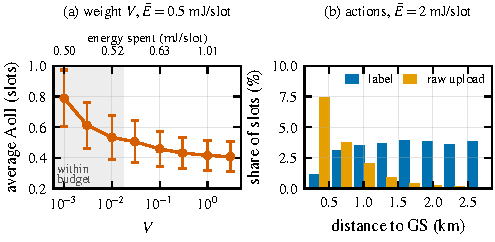
\includegraphics[width=\columnwidth]{figures/fig_V_mix.pdf}
\caption{(a) AoII of CA-DPP vs.\ $V$ at $\bar E=0.5$\,mJ/slot (top axis: energy spent; shaded: within $4\%$ of the budget). (b) Share of unblocked slots with a label or raw upload vs.\ distance to the GS, $\bar E=2$\,mJ/slot.}
\label{fig:Vmix}
\end{figure}

In Fig.~\ref{fig:Vmix}(a), at $0.5$\,mJ/slot, raising $V$ from $10^{-3}$ to $3$ lowers the AoII from $0.79$ to $0.41$, but the virtual queue builds up more slowly, and over a run of about $27{,}000$ slots the energy spent rises from $0.50$ to $1.51$\,mJ/slot. Values of $V$ up to $10^{-2}$ stay within $4\%$ of the budget. In Fig.~\ref{fig:Vmix}(b), at $2$\,mJ/slot and within $850$\,m of the GS, where uploads are cheap and reliable, CA-DPP uploads in $5.9\%$ of the unblocked slots and labels in $2.0\%$. Beyond $2.15$\,km it uploads in $0.1\%$ and labels in $3.8\%$.

%% =====================================================================
\section{Conclusion}\label{sec:concl}
%% =====================================================================
We studied status updates from a UAV whose sensor is its own classifier, tracking the GS's AoII through a belief that each label updates according to its confidence. This belief gives closed-form one-step values for the three actions and a drift-plus-penalty policy with confidence thresholds. On flood-mapping traces under chip-level cross-validation, the policy outperforms adaptations of three recent designs at every budget up to $5$\,mJ per slot. Against an AoII-threshold policy it helps when energy is scarce or the on-board classifier is weak, because then the confidence decides which disagreements are worth reporting. With an accurate classifier and ample energy, reporting every disagreement works as well, and a belief that knows only the precision of each label value matches one that uses the per-frame confidence.

On-board errors on overlapping footprints are correlated in time, and our belief handles this only through a tempered likelihood. A belief that models the correlation is the most promising way to improve the policy at large budgets. The one-step rule also does not anticipate predictable outages such as range limits or satellite passes, and the structure of the optimal POMDP policy and a performance bound for a renewal version still need proofs. Finally, Sentinel-2 imagery, generated separately from the UAV position, stands in for UAV frames. A spatial model of the area, with revisits and a route chosen by the UAV, is future work. Repeating the study with UAV datasets such as FLAME~\cite{shamsoshoara2021flame} and AIDER~\cite{kyrkou2020aider}, with energy measured on a microcontroller, is the next step.

\bibliographystyle{IEEEtran}
\bibliography{refs}

\end{document}
